\section{Muon Source}

\begin{figure}[h]
    \begin{center}
    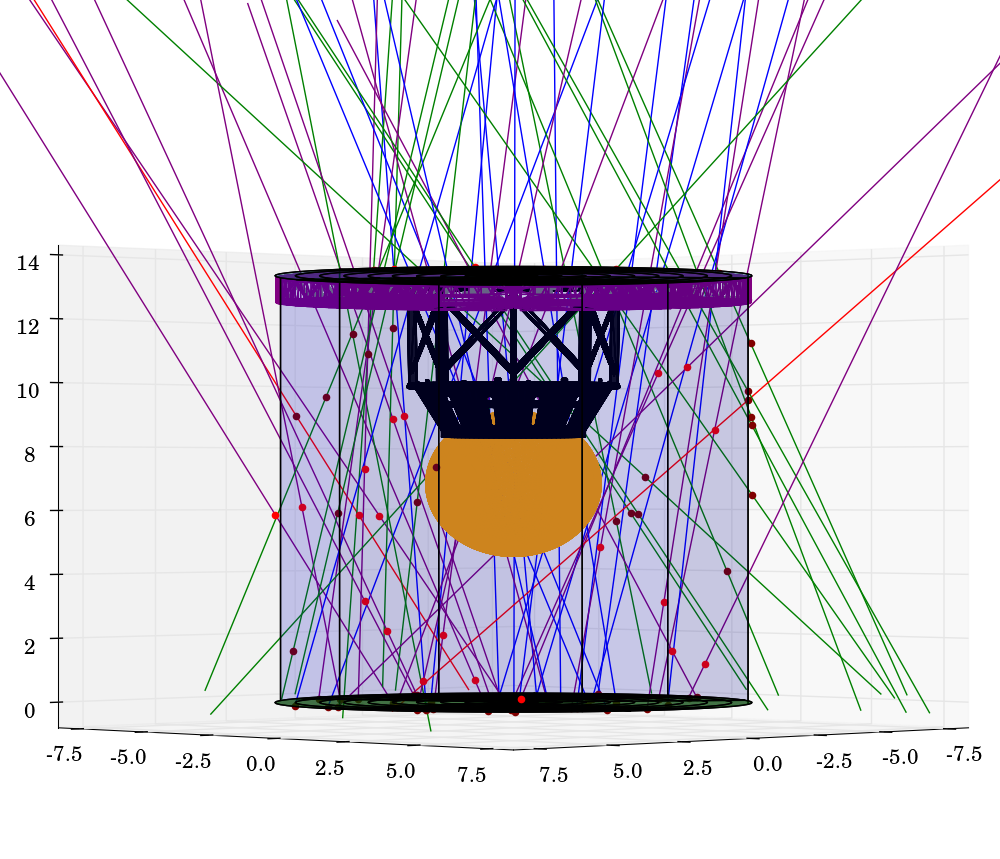
\includegraphics[scale=0.3]{figures/muons_1.png}
    \caption{A visualization of muons passing through a more sophisticated nEXO geometry}
    \label{fig:muons_1}
    \end{center}
\end{figure}

\paragraph{}
In FLUKA, one may define a beam-like source using the built-in \textcolor{Maroon}{BEAM} cards. However, if one wishes to simulate a more novel or complex series of source particles, a different user routine can do the trick. In the FLUKA literature and on the forums, this more complex source file is called ``source\_newgen.f''. In the simulation files here, it is called ``muon\_from\_file.f'' as this makes more sense. This user routine comes with a set of built-in functions allowing a sophisticated user to sample energies from various functions (Maxwell-Boltzmann for instance) and sample various initial positions. In our case, however, we only make use of a pair of features— the \textit{real} source generation is done with a more easily readable and modifiable set of python functions. To learn about how the muons are simulated, please see \cite{rross_muon_technote}.

\paragraph{}
In ``muon\_from\_file.f'' particles are read from a phase-space file (we'll get to that) and passed to FLUKA where they are propogated through the configuration and scored as requested. This is done using the built in routine ``read\_phase\_space\_file''. In this user routine, a file argument is provided pointing to the list of muons (called a phase space file). This is kept in the ``sim\_files'' directory and created with each run using the ``run\_simulation.py'' script (for now). The files are created externally using the muon\_functions.py module in the ``sim\_tools'' directory. Basically, the file contains a list of muons with attributes listed as comma-separated values in the following order:

\[
    \begin{matrix}
        \text{Particle No.} & \text{Energy  [GeV]} & X_0 \text{ [m]} & Y_0 \text{ [m]}& Z_0 \text{ [m]}& \cos(x) & \cos(y) & -\cos(z) & \text{Weight}
    \end{matrix}
\]

or equivalently in FLUKA language:

\[
    \begin{matrix}
        \text{JTRACK} & \text{ETRACK} & \text{XSCO} & \text{YSCO} & \text{ZSCO} & \text{CXTRCK} & \text{CYTRCK} & \text{CZTRCK} & \text{WTRACK}
    \end{matrix}
\]

\paragraph{}
The particle number (JTRACK) is either 10 (positive muon) or 11 (negative muon). These variables will be further discussed in the section on customized scoring. 

